\documentclass[12pt]{article}


% https://www.google.com/url?sa=t&rct=j&q=&esrc=s&source=web&cd=2&cad=rja&uact=8&ved=2ahUKEwj9gfHZp6ngAhV3VxUIHf1ZBpYQFjABegQICBAC&url=http%3A%2F%2Fwww.bens.ws%2Fpapers%2FSchoofElkiesAtkinAlgorithm.pdf&usg=AOvVaw3YjeZq80997dE-o0TE0vNI
% set font encoding for PDFLaTeX or XeLaTeX
\usepackage{ifxetex}
\ifxetex
  \usepackage{fontspec}
\else
  \usepackage[T1]{fontenc}
  \usepackage[utf8]{inputenc}
  \usepackage{a4wide}
  \usepackage{lmodern}
  \usepackage[french]{babel}
  \usepackage{amsmath,amsfonts,amssymb,amsthm,epsfig,epstopdf,titling,url,array,amssymb}
  \usepackage{graphicx}
  \usepackage{caption} 
  \usepackage{array}
  \usepackage{graphics,graphicx}
  \usepackage[usenames,dvipsnames]{pstricks}
  \usepackage{calc}
  \usepackage{multirow}
  \usepackage{algorithmic}
  \usepackage{algorithm}
  \usepackage{appendix}
  \usepackage{stmaryrd}
  \usepackage{calrsfs}
  \usepackage{tikz}
  \usepackage{pgfplots}
  \usepackage{mathabx}
%  \usepackage{boondox-cal}
  \usepackage{tikz}  
  \usetikzlibrary{decorations.pathmorphing}
  \usetikzlibrary{decorations.pathreplacing}
  \usetikzlibrary{decorations.shapes}
  \usetikzlibrary{decorations.text}
  \usetikzlibrary{decorations.markings}
  \usetikzlibrary{decorations.footprints}
  \usepackage{color}
  \usepackage{geometry}
	\geometry{hmargin=2.5cm,vmargin=2cm}
  \usepackage{varioref}
  \usepackage{listings}
  
%  \usepackage[obeyspaces]{url}


  \lstdefinelanguage{Sage}[]{Python}
  {morekeywords={False,sage,True},sensitive=true}
	\lstset{frame=none,
  showtabs=False,
  showspaces=False,
  showstringspaces=False,
  commentstyle={\ttfamily\color{dgreencolor}},
  keywordstyle={\ttfamily\color{dbluecolor}\bfseries},
  stringstyle={\ttfamily\color{dgraycolor}\bfseries},
  language=Sage,
  basicstyle={\fontsize{10pt}{10pt}\ttfamily},
  aboveskip=0.3em,
  belowskip=0.1em,
  numbers=none,
  numberstyle=\footnotesize,
}
\definecolor{dblackcolor}{rgb}{0.0,0.0,0.0}
\definecolor{dbluecolor}{rgb}{0.01,0.02,0.7}
\definecolor{dgreencolor}{rgb}{0.2,0.4,0.0}
\definecolor{dgraycolor}{rgb}{0.30,0.3,0.30}
\newcommand{\dblue}{\color{dbluecolor}\bf}
\newcommand{\dred}{\color{dredcolor}\bf}
\newcommand{\dblack}{\color{dblackcolor}\bf}

\fi

% $\genfrac(){}{0}{a}{b}$


% used in maketitle
\title{Compter les points sur une courbe elliptique}
\author{Jérémie Coulaud}

% Enable SageTeX to run SageMath code right inside this LaTeX file.
% documentation: http://mirrors.ctan.org/macros/latex/contrib/sagetex/sagetexpackage.pdf
%\usepackage{sagetex}

\graphicspath{{../pictures/}}
\DeclareMathOperator{\e}{e}
\def\Tr{\mathop{\rm{Tr}}\nolimits}
\def\bwp{{\bar \wp}}
\def\bwp{{\bar {\wp'}}}
\begin{document}

\newtheorem{prop}{Proposition}
\newtheorem{defi}{Définition}
\newtheorem{thm}{Théorème}
\maketitle
\newpage
\tableofcontents
\newpage

\section{Introduction}
La cryptographie sur courbe elliptique introduite en 1985 a révolutionné la cryptographie à clé publique permettant une alternative efficace aux classique RSA et Diffie Hellman. Les courbes elliptiques sont énormément utilisées pour les signatures (ECDSA), notamment pour le Bitcoin, et supportées dans la majorité des applications TLS, SSH. La sécurité d'un cryptosystème basé sur les courbes elliptiques dépend du nombre de points rationnels de la courbe. Il est donc intéressant de trouver des algorithmes efficaces pour déterminer ce nombre dans le but de construire des courbes elliptiques utilisable en cryptographie.
Le but de ce rapport est de présenter des algorithmes pour compter les points sur une courbe elliptique et de les implémenter pour tester leur efficacité. Après une brève introduction à la théorie de base des courbes elliptiques on va décrire l'algorithme de Schoof, qui est polynomial mais peu efficace en pratique. Dans la suite on va essayer de comprendre les amélioration faites à cet algorithme par Atkins et Elkies conduisant a un algorithme toujours polynomial mais beaucoup plus efficace.
\newline
L'ensemble des codes est disponible sur le github \url{https://github.com/bialx/Elliptic-Curve-} Le langage choisi est SAGE, basé sur Python. Il contient un large éventail de fonctions mathématiques prédéfinies, notamment pour les courbes elliptiques ce qui permet de se concentrer sur les algorithmes et non sur une implémentation d'objets mathématiques.
\section{Introduction aux courbes elliptiques}
 On se contentera de donner une explication succincte de ce qu'est une courbe elliptique ainsi que différentes propriétés associées.

\begin{defi}
On définit une courbe elliptique sur un corps $K$ dans un plan par une équation de Weierstrass de la forme : 
\begin{equation*}
y^2 + a_1xy + a_3y  = x^3 + a_2x^2 + a_4x + a_6
\end{equation*}
Les coefficients $a_{1 \leq i \leq 6}$ sont des éléments du corps $K$.
\end{defi}

Dans le cas où le corps $K$ a une caractéristique différente de $2$ ou $3$ on peut, via des changements de variable se ramener à l'équation courte suivante : 
\begin{equation*}
y^2 = x^3 + ax +b
\end{equation*}

\begin{defi}
Soit $E : y^2 = x^3 + ax +b$ une courbe sur $K$ on pose : 
\begin{equation*}
\Delta = -16*(4a^3 + 27b^2) \quad \text{et} \quad j(E) = \frac{(-48a)^3}{\Delta}
\end{equation*}
$\Delta$ est appelé le discriminant de $E$, et $j(E)$ son j-invariant. La courbe $E$ est une courbe elliptique si et seulement si $\Delta \ne 0$.
\end{defi}

\begin{defi}
L'ensemble des points de la courbe $E$ est noté $E(K)$ avec :
\begin{equation*}
E(K) = \left\{ (x,y) \in \mathbb{K} \, | \, y^2 + a_1xy + a_3y  = x^3 + a_2x^2 + a_4x + a_6 = 0_E \right\} \cup {O}
\end{equation*}
Où $O$ est le point à l'infini
\end{defi}


On peut définir une loi de groupe abélien $\oplus$ sur $E(K)$ de neutre le point à l'infini $O$. On a pour tout $P = (x,y) $ dans $E(K)$ donnée sous forme réduite:
\begin{itemize}
\item[(1)] $O \oplus (x,y) = (x,y) \oplus O = (x,y)$
\item[(2)] $\ominus (x,y) = (x, -y)$
\item[(3)] Soit $P,Q,R \in E(K)$, si ces trois points sont alignés alors $P \oplus Q \oplus R = 0$
\end{itemize}

Maintenant qu'on a donné une structure de groupe abélien à $E(K)$ on peut donner des formules explicites d'addition de points sur la courbe.

\begin{prop}
Soit $P =(x_1, y_1), Q=(x_2, y_2)$.
$$P \oplus Q = (x_3, y_3) = (\lambda^2 -x_1 -x_2, \lambda(x_1 - x_3 - y_1)) $$
En posant : 

\begin{equation}
\lambda =
\left\lbrace
\begin{array}{ccc}
\frac{y_2 - y_1}{x_2 - x_1} & \mbox{si} & P \ne Q, -Q  \\
\frac{3x^2 + a}{2y_1} & \mbox{si}  & P = Q, y_1 \ne 0
\end{array}\right.
\end{equation}
\end{prop}

\begin{figure}[h!]
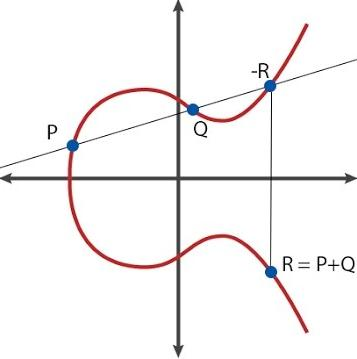
\includegraphics[scale=0.7]{pictures/hqdefault.jpg} 
\caption{vision graphique de l'addition de deux points sur la courbe}
\end{figure}


On dispose de formule d'addition pour deux points sur une courbe elliptique on peut donner un sens à la multiplication scalaire d'un point comme $lP = \underbrace{P + \ldots + P}_{l \text{ fois}}$. On va noter cette multiplication scalaire par :
\newline

$\begin{array}{ccccc}
[l]_E & : & E(\mathbb{K}) & \to & E(\mathbb{K}) \\
 & & P & \mapsto & lP\\
\end{array}$

Ce qui nous permet de définir l'ensemble des points de $l$-torsion comme le noyau de $[l]$. On note $E[l]$ cet ensemble.
\newline
$$E[l] = \left\{ P \in E(\overline{\mathbb{K}}) \, | \, [l]P = 0_E \right\} $$

\section{Compter les points sur une courbe}
On va considérer dans la suite que la caractéristique du corps utilisé pour définir nos courbes elliptiques est plus grande que $3$. On peut donc écrire notre courbe elliptique sur $\mathbb{F}_p$ sous sa forme réduite $y^2 = x^3 + ax+b$

\subsection{Algorithme naïf}
On note $E: y^2 = f(x)$, compter les points de $E$ revient donc pour chaque valeur de $x \in \mathbb{F}_p$ à regarder si $f(x)$ est un carré modulo $p$. On calcule donc le symbole de Legendre de $f(x)$, on a les cas suivants : 
\begin{itemize}
\item  $\genfrac(){}{0}{f(x)}{p} = -1$, $f(x)$ n'est pas un carré modulo $p$, on ne trouve aucun point appartenant à la courbe.
\item $\genfrac(){}{0}{f(x)}{p} = 0$, $f(x)$ est divisible par $p$, on trouve $1$ point sur la courbe.
\item $\genfrac(){}{0}{f(x)}{p} = 1$, $f(x)$ est un carré modulo $p$, on trouve $2$ points sur la courbe.
\end{itemize}
\medskip
Au final en considérant le point à l'infini on peut calculer le nombre de points de $E$ : 
\begin{equation*}
\#E(\mathbb{F}_p) = 1 + \sum_{x \in \mathbb{F}_p}(\genfrac(){}{0}{f(x)}{p} + 1)
\end{equation*}
Soit : 
\begin{equation}
\#E(\mathbb{F}_p) = 1 + p +\sum_{x \in \mathbb{F}_p}\genfrac(){}{0}{f(x)}{p}
\end{equation}
On peut implémenter cette fonction brute force très simplement sous sage en utilisant \path{kronecker(a,p)} qui calcule le symbole de Legendre de $a$ modulo $p$.
\medskip
\begin{lstlisting}
def brute_force(p, a,b):
    R.<x> = PolynomialRing(GF(p))
    f = x**3 + a*x + b
    return 1+p+sum([kronecker(f(i),p) for i in range(p)])

\end{lstlisting}

\bigskip
La complexité est en la taille de $p$. Cette méthode est pratique quand $p$ est petit mais devient impraticable s'il est trop grand.
On va illustrer la non efficacité de cet algorithme lorsque $p$ devient trop grand par le graphique suivant:

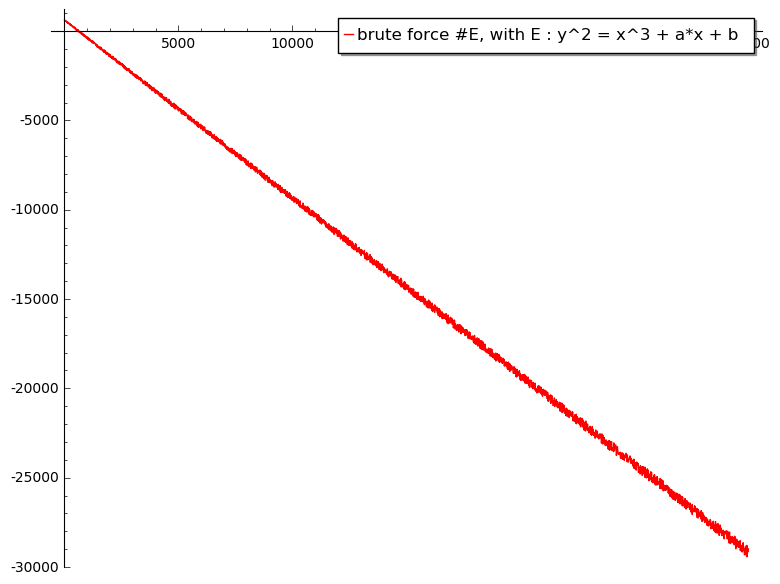
\includegraphics[scale=0.5]{pictures/brute_force_cputime.png} 

On retrouve bien l'aspect linéaire en $p$ évoqué précédemment.
\subsection{Shanks}
Il s'agit d'un algorithme Baby steps-giant steps de complexité exponentielle qu'on ne traitera pas ici, mais plus d'informations peuvent être trouvées ici \cite{artSchoof}

\subsection{Schoof}
Soit $E$ une courbe elliptique définie sur $\mathbb{F}_p$ avec $p$ premier $>3$ sous sa forme réduite 
$$ E: y^2 = x^3 + ax+b$$
On rappelle le théorème de Hasse-Weil:

\begin{thm}
$\#E(\mathbb{F}_p) = p + 1 - t$ avec $|t| \leq 2 \sqrt{p}$ trace de l'endomorphisme de Frobenius de $E$.
\end{thm}
Pour trouver le nombre de points de $E$ il faut donc déterminer $t$. 
L'idée de Schoof est de calculer $t$ modulo de petits nombres premiers puis d'utiliser le théorème des restes chinois. 

Avant de développer l'algorithme il est nécessaire de donner d'autres définitions. 

\begin{defi}[Frobenius]
Soit $E$ une courbe elliptique défini sur $\mathbb{F}_p$, l'endomorphisme de Frobenius est défini par 

$\begin{array}{ccccc}
\phi_p & : & E(\mathbb{F}_p) & \to & E(\mathbb{F}_p) \\
 & & (x,y) & \mapsto & (x^p, y^p) \\
\end{array}$
\end{defi}
On peut définir le polynôme caractéristique de cet endomorphisme par $\phi_p^2 - t \phi_p + p = 0$.
On peut déjà faire une première remarque, connaissant $t$ la trace de l'endomorphisme de Frobenius, $E$ une courbe elliptique sur $\mathbb{F}_p$, il est facile de déterminer le cardinal de $E(\mathbb{F}_{p^n}$) pour tout $n >1$. En effet on a :
\begin{equation*}
\#E(\mathbb{F}_{p^n}) = p^n + 1- (r_1^n + r_2^n)
\end{equation*}
où $r_1, r_2$ sont les racines de $x^2 - tx +p$ dans $E(\mathbb{F}_{p^n})$, le polynôme caractéristique du Frobenius.
\begin{proof}
Les racines de $x^2 - tx +p$ sont $r_1$ et $r_2$, on a donc $\Tr(\phi_p) = t = r_1 + r_2$. 
\newline
On remarque de plus que l'on a $\phi_{p^n} = (\phi_p)^n$. Car $\phi_{p^n} (x,y) = (x^{p^n}, y^{p^n}) = \phi_p  (x^{p^{n-1}}, y^{p^{n-1}})$, et par récurrence on trouve le résultat).
\newline
Ainsi : 
\begin{align*}
\Tr(\phi_{p^n} (x,y)) &= \Tr(\phi_{p} (x,y)^n) \\
					 &= r_1^n + r_2^n	 
\end{align*}
On peut maintenant appliquer le théorème de Hasse-Weil pour trouver le résultat attendu.
\end{proof}

L'équation du polynôme caractéristique du Frobenius reste en particulier vraie sur les points de $l$-torsion, ce qui nous sera utile par la suite. Ainsi nous avons : 
\begin{equation}
\label{eqnfrobenius}
 \phi_p^2(P)  + [p_l]P = [t_{l}] \phi_p(P) \quad \forall P \in E[l]
\end{equation} 
Avec $t_l \equiv t \pmod l$, $p_l \equiv p \pmod l$ et $0 \leq t_l, p_l < l$. 
\newline
Il nous faut maintenant introduire les polynômes de division d'une courbe elliptiques $E$.

\begin{defi}
Soit une courbe elliptique $E : y^2 = x^3 + ax+b$ défini sur $\mathbb{K}$. On appelle $f_n(X)$ le n-ième polynôme de divisons défini sur $\mathbb{Z}[x]$ de manière récursive par : 


\begin{align*}
f_0(x) &= 0 \\
f_1(x) &= 1 \\
f_2(x) &= 1 \\
f_3(x) &= 3x^4 + 6ax^2 +12bx - a^2 \\
f_4(x) &= 2x^6 + 10ax^4 +40bx^3 - 10a^2x^2 - 8abx - 2(a^3 + 8b^2)
\end{align*}
On pose $F(X)= 4x^3 + 4ax + 4b$, et on a:

\begin{equation}
\left\lbrace
\begin{array}{ll}
f_{2n}& =  f_n(f_{n+2}f_{n-1}^2 - f_{n-2}f_{n+1}^2)   \\
f_{2n+1}& = \left\lbrace 
\begin{array}{ccc}
F^2f_{n+2}f_n^3 - f_{n-1}f_{n+1}^3 & \mbox{si} & n \text{ est pair}\\
f_{n+2}f_n^3 - f_{n-1}f_{n+1}^3F^2 & \mbox{si} & n \text{ est impair} \end{array}\right.

\end{array} \right.
\end{equation} 
Ces polynômes sont de degrés au plus $\frac{(n^2 -1)}{2}$ si $n$ est pair, ou bien  au plus $\frac{(n^2 -2)}{2}$ si $n$ est impair.
\end{defi}


On peut utiliser les polynômes de division pour calculer la multiplication scalaire d'un point de la courbe $E$.
On a les formules suivantes : 

\begin{thm}
Soit $E$ une courbe elliptique défini sur $\mathbb{K}$, un point $P$ sur cette courbe et $m \in \mathbb{N}^*$.

\begin{equation}
[m]P = 
\left\lbrace
\begin{array}{ccc}
O_E & \mbox{si} & P \in E[m]  \\
\left(    \frac{\phi_m(x,y)}{\psi^2_m(x,y)}, \frac{\omega_m(x,y)}{\psi^3_m(x,y)}\right) & \mbox{sinon}  & 
\end{array}\right.
\end{equation}

En posant : 
\begin{equation*}
\psi_m= \left\lbrace
\begin{array}{cc}
2yf_m & \mbox{si m est pair} \\
f_m & \mbox{sinon}
\end{array}\right.
\end{equation*}
et 
\begin{equation*}
\left\lbrace
\begin{array}{ll}
\phi_m &= x \psi^2_m - \psi_{m-1}\psi_{m+1} \\
\psi_m \omega_m &= \psi_{2m}
\end{array}\right.
\end{equation*}
On peut aussi réécrire $[m]P$ sous cette forme : 
\begin{equation}\label{mP}
[m]P = \left\lbrace
\begin{array}{lll}
O_E & \mbox{si} & P \in E[m]  \\
\left(  x -   \frac{\psi_{m-1}(x,y)\psi_{m+1}(x,y)}{\psi^2_m(x,y)}, \frac{\psi_{2m}(x,y)}{\psi^4_m(x,y)}\right) & \mbox{sinon}  & 
\end{array}\right.
\end{equation}
\end{thm}

\begin{proof}
On veut démontrer l'équation \ref{mP}. 
\newline
On note $[m]P = (x_1, y_1)$ 
On a alors : 

\begin{align*}
y_1 &= \frac{\omega_m}{\psi^3_m} = \frac{\psi_{2m}}{\psi_m} \frac{1}{\psi_m^3} = \frac{\psi_{2m}}{\psi_m^4} \\
x_1 &= \frac{\phi_m}{\psi^2_m} =  \frac{x \psi^2_m - \psi_{m-1}\psi_{m+1}}{\psi_m^2} = x - \frac{\psi_{m-1}\psi_{m+1}}{\psi_m^2}	
\end{align*}




\end{proof}
On remarque que $[m]P = (x_1, y_1)$ avec $x_1$ uniquement fonction de $x$. En effet en utilisant les formules de récurrence, si $m$ est pair $\psi_m^2 = 4y^2f_m$, mais en utilisant l'équation de $E$ on peut remplacer $y^2$ par une fonction de $x$, et les polynômes de division sont en fonction de $x$. De plus comme $m$ est pair les polynômes $\psi_{m+1} et \psi_{m-1}$ sont uniquement en fonction de $x$. Dans le cas où $m$ est impair on a l'inverse, le numérateur fait apparaître un $y^2$ qu'on peut remplacer par une fonction de $x$ comme précédemment et le dénominateur est une fonction de $x$. Quand à $y_1$, son degré en $y$ est au plus $1$. Si $m$ est pair $\psi_m^4$ fait apparaître un $y^4$ qui s'exprime en fonction de $x$, et $\psi_{2m}$ amène un $y$. On montre la même chose quelque soit la parité de $m$ et $2m$.
On peut ainsi exprimer $[m]P$ comme un polynôme en $x,y$. Mais ce n'est pas la seule particularité de ces polynômes utiles pour notre algorithme. En effet $P = (x_1, y_1)$ est un point de $l$-torsion si et seulement si $x_1$ est une racine du $l$-ième polynôme de division $f_l$. De plus $P$ est sur la courbe $E$. Les points de $l$-torsion sont donc solutions du système d'équation : 
\begin{equation}
E(x,y) = y^2 - x^3 - ax - b = 0, \quad f_l(x) = 0
\end{equation}
L'équation \ref{eqnfrobenius} peut donc se récrire en utilisant les points de $l$-torsion. On va maintenant faire des calculs dans l'anneau
$$\mathbb{W}= \frac{\mathbb{F}_p[x,y]}{(f_l(x), E(x,y))}$$
L'idée de l'algorithme de Schoof est donc de tester pour des valeurs $\tau_l \in \lbrace 0, \ldots, l-1 \rbrace$ si l'équation suivante est vraie dans cet anneau :

\begin{equation}
(x^{p^2}, y^{p^2}) + [p_l](x,y) = [\tau_l](x^{p}, y^{p}),  \quad P=(x,y)
\end{equation}
L'unique solution que l'on trouve est $t_l$.On répète l'opération pour d'autres $l$ premiers jusqu'à avoir assez de $t_l$ pour appliquer le théorème des restes chinois et retrouver la valeur de $t$. L'intérêt de travailler avec des points de $l$-torsion est ainsi de pouvoir borner la taille des polynômes en jeu dans l'équation du Frobenius, en $O(l^2)$, ce qui est plus efficace que de uniquement travailler avec des fonctions rationnelles.
\newline
\medskip
On va maintenant détailler l'algorithme étape par étape. 


\subsubsection{Choix de l'ensemble de premiers}
L'idée de Schoof est de calculer la trace de l'endomorphisme de Frobenius modulo de petits premiers. Il faut choisir un ensemble $S = (l_1, \ldots l_n)$ tel que $\prod l_i > 4\sqrt{p}$. En effet on rappelle que  $|t| \leq 2 \sqrt{p}$, on veut s'assurer de bien pouvoir reconstruire notre solution quand on va utiliser les restes chinois. Pour construire $S$ on va juste ajouter des nombres premiers à une liste en utilisant la fonction \path{next_prime} de SAGE tant que le produit des éléments de $S$ est plus petit que $ 4\sqrt{p}$. Au final cela revient à la boucle suivante OU $n$ est initialisé à $1$ et \path{list_l} correspond à $S$:
\bigskip

\begin{lstlisting}
while N <= 4*sqrt(p):
	if prime == p:
		pass
	prime = next_prime(prime)
	N = N*prime
	list_l.append(prime)
\end{lstlisting}


\subsubsection{Cas $l=2$}
Ce cas est particulier et doit être traité à part car on suppose nos premiers impairs. On a $t_2 \equiv 0 \pmod 2$ si et seulement si $E(\mathbb{F}_p)$ a un élément d'ordre $2$, c'est à dire un point de $2$-torsion. Or les points de $2$ torsions sont de la forme $(x, 0)$. En effet, si $2P = 0$, pour $P \in E(\mathbb{F_p})$ alors $P = -P$, et cela correspond aux points de l'axe des abscisses. Ainsi $t_2$ est congru à $0$ si et seulement si $x^3 +ax +b$ à une racine dans $\mathbb{F}_p$. Mais les racines de $\mathbb{F}_p$ sont entièrement déterminées par le polynôme $x^p - x$, nos deux polynômes partageraient alors une racine commune. La façon utilisée ici pour décider si $t_2 \equiv 0 \pmod 2$ est donc de calculer si $\gcd(x^p - x, x^3 +ax +b) \ne 1$ (qu'on calcule par exponentiation rapide).

\subsubsection{Calcul des polynômes de division}
Il existe dans SAGE une fonction permettant de calculer les polynômes de division, \path{polynomial_polynomial(n)} renvoyant le $n$-ième polynôme de division. Mais comme au cours de l'algorithme on doit souvent utiliser différents polynôme de division et de plus ils sont calculés via des formules de récurrence. Il ne me paraissait pas forcement très judicieux d'utiliser la fonction de sage qui allait de toute façon très certainement à chaque appel devoir recalculer via les formules de récurrence le polynôme souhaité. L'idée étant de stocker tous ces polynômes dans un dictionnaire, une fois la phase de pré calcul faite on peut donc accéder à tous les polynômes de division que l'on souhaite en temps constant au cours de l'exécution de l'algorithme de Schoof. Et en utilisant la fonction de SAGE j'ai tout de même vérifié via une fonction de test que je trouvais bien les même polynômes qu'avec ma fonction.


\subsubsection{Calcul de $(x^{p^2}, y^{p^2}) + [p_l](x,y)$}

Comme vu en introduction aux courbes elliptiques la somme de deux points appartenant à la courbe dépend de plusieurs cas. Est-ce que nos points sont distincts ou ont la même coordonnée en $x$. En effet les formules à appliquer seront différentes selon que l'on soit dans un cas ou l'autre. Il est plus probable d'avoir des coordonnées différentes, on va donc travailler dans ce cas là. Si l'algorithme trouve un $t_l$ vérifiant l'équation on est dans le bon cas, s'il n'en trouve aucun, cela veut dire que l'on se trouve dans l'autre cas.
\paragraph*{Cas : $(x^{p^2}, y^{p^2}) \ne \pm [p_l](x,y)$}

On peut utiliser notre formule usuelle d'addition sur courbe elliptique pour calculer $(x_1, y_1) = (x^{p^2}, y^{p^2}) + (x_{\bar{p_l}}, Y_{\bar{p_l}})$ en notant $(x_{\bar{p_l}}, y_{\bar{p_l}}) =  [p_l](x,y)$. 
\newline
Soit $\lambda = \frac{y_{\bar{p_l}} - y^{p^2}}{x_{\bar{p_l} - x^{p^2}}}$, on a alors :
\begin{equation}
(x_1, y_1) = (\lambda^2 - x^{p^2} - x_{\bar{p_l}}, \, \lambda (x^{p^2} - x_1) -  y^{p^2})
\end{equation}
On va aussi noter $(x_{\tau}, y_{\tau}) =  [\tau](x,y)$. On doit maintenant tester en faisant varier la valeur de $\tau$ entre $0$ et $\frac{l-1}{2}$ si $x_1 = x_{\tau}$. Si c'est le cas on se retrouve avec deux possibilités comme valeur de $y_1$, soit on a le point soit on a son opposé. On regarde donc si $y_1 = y_{\tau}$, on a alors $t_l = \tau$, sinon on a $t_l = - \tau$

\paragraph*{Cas : $(x^{p^2}, y^{p^2}) = \pm [p_l](x,y)$}
Là encore deux cas possibles. On va d'abord regarder lorsque $(x^{p^2}, y^{p^2}) = [p_l](x,y)$. 
\newline
Soit $P=(x,y)$, on rappelle l’équation caractéristique de l'endomorphisme Frobenius restreinte aux points de $l$-torsion: 
\begin{equation}
\phi_p^2(P)  + [p_l]P = [t_{l}] \phi_p(P) \quad \pmod{l}
\end{equation}
On a alors dans notre cas $2[p_l]P = [t_{l}] \phi_p(P) \, \pmod{l}$. De plus on a $\phi_p^2 = [p_l]P$. En combinant ces deux égalités on trouve :

\begin{equation}
[t_l^2 p_l]P = [t_l^2] \phi_p^2 = [t_l] \phi ([t_l] \phi_p) = [(2p_l)^2]P \quad \pmod{l}
\end{equation}
Ainsi $p_l$ est un carré modulo $l$. On pose $p_l = \omega^2 \pmod{l}$. On va maintenant calculer $\omega \phi P$, si $[p_l]P = \omega \phi P$ alors $t_l = 2\omega$ sinon $t_l = -2\omega$.
\newline
\medskip
Si $p_l$ n'est pas un carré modulo $l$ on est dans le cas $(x^{p^2}, y^{p^2}) = - [p_l](x,y)$ et on a alors $t_l = 0$ d'après l'équation caractéristique. 

\newpage
\subsubsection{Algorithme}
On donne une version complète en pseudo-code de l'algorithme de schoof : 

\begin{algorithm}
\caption{Schoof}
\begin{algorithmic}
\REQUIRE $E$ une courbe elliptique de la forme $y^2 = x^3 + ax = b$ sur $\mathbb{F}_p$
\ENSURE Le nombre de points de $E$

\STATE Choisir un ensemble de premier S tel que $\prod_{l \in S}l \leq 4\sqrt{p}$
\IF{$\gcd(x^q - x, x^3 + ax +b) \ne 1$} 
\STATE $t_2 = 0$
\ELSE
\STATE $t_2 = 1$
\ENDIF

\FORALL{$l \in S$}
\STATE Calculer le polynôme de division $f_l$, on fera les calculs dans l'anneau $\mathbb{F}= \frac{\mathbb{F_p}[X,Y]}{(f_l(X), y^2 -x^3 - ax - b})$
\STATE On pose $p_l = p \mod(l)$
\STATE Calculer $(x^p, y^p), \, (x^{p^2}, y^{p^2}), \, [p_l](x, y) = (x_{p_l}, y_{p_l})$
\IF{$x^{p^2} \ne  x_{p_l}$}
\STATE Calculer $(X, Y) = (x^{p^2}, y^{p^2}) + (x_{p_l}, y_{p_l})$
\FORALL{$1 \leq \tau \leq l - 1$}
\IF{$X = x^p_{\tau}$}
\IF{$Y = y^q_{p_l}$}
\STATE $t_l = \tau$
\ELSE 
\STATE $t_l = - \tau$
\ENDIF
\ENDIF
\ENDFOR
\ELSE
\IF{$p$ est un carré modulo $l$}
\STATE Calculer $w$ tel que $p \equiv w^2 \pmod l$ 
\STATE Calculer $[w](x^p,y^p)]$
\IF{$[w](x^p,y^p)] = (x^{p^2}, y^{p^2})$}
\STATE $t_l = 2w$
\ENDIF
\IF{$[w](x^p,y^p)] = (x^{p^2}, -y^{p^2})$}
\STATE $t_l = -2w$
\ELSE
\STATE $t_l =0$
\ENDIF
\ELSE
\STATE $t_l = 0$

\ENDIF
\ENDIF
\ENDFOR
\end{algorithmic}
\end{algorithm}
\newpage

\paragraph*{Implémentation}
Il a fallut commencer par implémenter des fonctions de base sur les courbes elliptiques pour additionner, calculer une multiplication scalaire. Les algorithmes d'additions ne nécessitent pas d'explications, juste une application des formules. Pour la multiplication scalaire on avait deux choix, utiliser les polynômes de division ou de l'exponentiation rapide. La méthode utilisant les polynômes a amené des problème d'implémentation, notamment pour faire les calculs dans les bons anneaux, donc je suis resté avec une version plus simple d'exponentiation. L'idée de cet algorithme est d'utiliser la décomposition binaire de $n$ pour calculer $nP$. Pour récupérer cette décomposition on utilise la fonction \path{digits(base)} qui retourne une liste avec les bits de poids faible à gauche de l'écriture binaire de $n$. On va à chaque itération doubler le point que l'on a, on calcule donc $2(2(\ldots2(P))$. Il est même nécessaire lorsque l'on rencontre un $1$ dans la décomposition binaire de $n$ de faire une addition en plus de doubler. Au final on obtient l'algorithme suivant avec comme entre $n$ et $P$: 
\bigskip
\begin{lstlisting}
    nbits = n.digits(2)
    i = len(nbits)-2
    Q = P
    while i >= 0:
        Q = double(Q,a)
        if nbits[i]:
          Q = add(P,Q,a)
        i -= 1
    return Q
\end{lstlisting}
\bigskip

Sans donner ici le détail complet de l'algorithme sous SAGE il est intéressant de détailler certains points de l'implémentation. Le premier soucis rencontré fut la construction de l'anneau dans lequel on doit travailler. On crée tout simplement un anneau de polynôme dans le corps $K$ pour commencer :
\bigskip
\begin{lstlisting}
R.<x> = PolynomialRing(K)
\end{lstlisting}
\bigskip
En notant \path{poly_divi_l} le $l$-ième polynome de division on peut construire l'anneau quotient : 
\bigskip

\begin{lstlisting}
B.<x2> = R.quotient(ideal(poly_divi_l))
\end{lstlisting}
\bigskip
Cependant on n'est pas certain que ce polynôme soit irréductible, et ainsi créer un corps fini. Si ce n'est pas le cas et que l'on doit calculer l'inverse d'un élément non inversible, on rencontrera une erreur. Il est donc nécessaire de tester si le polynôme de division est irréductible et s'il ne l'est pas de le remplacer par un de ses diviseurs. Ce qu'on illustre avec la condition suivante :
\bigskip
\begin{lstlisting}
if not poly_divi_l.is_irreducible():      
	for poly, deg in list(factor(poly_divi_l)):
		if deg > 1:
		poly_divi_l  = poly
		break
\end{lstlisting}
\bigskip

Une fois que cela est fait on peut, en notant $f=x^3 +ax+b$, créer l'anneau final :
\bigskip
\begin{lstlisting}
B.<x2> = R.quotient(ideal(poly_divi_l))
C.<y> = PolynomialRing(B)
W = C.quotient(y**2 - f)
\end{lstlisting}
\bigskip
Les calculs pour obtenir les différents $t_l$ modulo $l$ sont juste une succession de test comme décrit dans l'algorithme en pseudo-code. Il faut juste faire attention à bien faire les calculs dans le bon anneau.
Une fois que l'on a calculé une liste \path{list_t} contenant tous les $t$ modulo $l$ calculés par l'algorithme on peut utiliser la fonction de sage \path{crt(list_t, list_l)} renvoyant la valeur de $t$ final en utilisant les restes chinois.
\subsubsection{Exemple}
On va travailler avec la courbe $E$ suivante, $E$ : $y^2 =x^3 +2x+1$ sur $\mathbb{F}_{19}$.

\paragraph{$\mathbf{l=2}$}
On calcule $\gcd(x^{19} -x, x^3 + 2x+1)$ et on trouve $1$, donc $t \equiv 1 \pmod 2$

\paragraph{$\textbf{l=3}$}
On a $p^2 = 361$ et $p_l \equiv 1 \pmod 3$, on pose ainsi $p_l = 1$. L'équation du Frobenius devient : 
\begin{equation}
(x^{361}, y^{361}) + (x,y) = [\tau_l](x^{19}, y^{19})  \quad (x,y) \in E[3], \, \tau_l = \pm 1
\end{equation}
Le troisième polynôme de division est $f_l = 3x^4 + 12x^2 +12x - 4$ mais ce polynôme n'est pas irréductible dans $\mathbb{F}_{19}$, on va plutôt travailler avec un de ses diviseurs : $x^3 + 8x^2+16$.
\newline 
Il nous faut maintenant calculer la partie gauche de cette équation.
On a $x^{361} = 3x^2 +2x +5 \pmod f_{l}$ et $y^{361} = y(y^2)^{180} = y(4x^2+9x+16)$. On est dans le cas ou $x^{361} \ne x$. On doit maintenant utiliser nos formules de sommations pour calculer $(x_3, y_3) =(x^{361}, y^{361}) + (x,y)$ : 

\begin{align*}
x_3 &= (\frac{y(4x^2+9x+16) - y}{3x^2 +2x +5 - x})^2 -3x^2 -2x - 5 - x 
 	&= (y(4x^2+9x+15)(x^2+15x+6))^2 -3x^2 -3x - 5 \\
 	&= 11 - 3x^2 -3x - 5  \\
 	&= 16x^2 + 16x + 6 
\end{align*}
et, 

\begin{align*}
y_3 &= \frac{y(4x^2+9x+16) - y}{3x^2 +2x +5 - x} (4x^2+9x+16 -  16x^2 - 16x - 6) - y(4x^2+9x+16) \\
	&= y(4x^2+9x+15)(x^2+15x+6)( -12x^2 - 7x +10 ) - y(4x^2+9x+16)\\
	&= y(13x^2 + 13x + 14)
\end{align*}

Maintenant nous devons calculer pour $\tau$ variant de $0$ à $2$ si $(x_3, y_3) = \tau (x^p, y^p)=(x_{\tau}^p, y_{\tau}^p)$. Pour $\tau = 1$ on trouve $x_3 = x_{\tau}^p$ et $y^p= - y_{\tau}^p$. Ainsi $t_3 = -\tau = -1 = 2 \pmod 3$. 

\newpage
\subsubsection{Expérimentations}

\begin{figure}[h!]
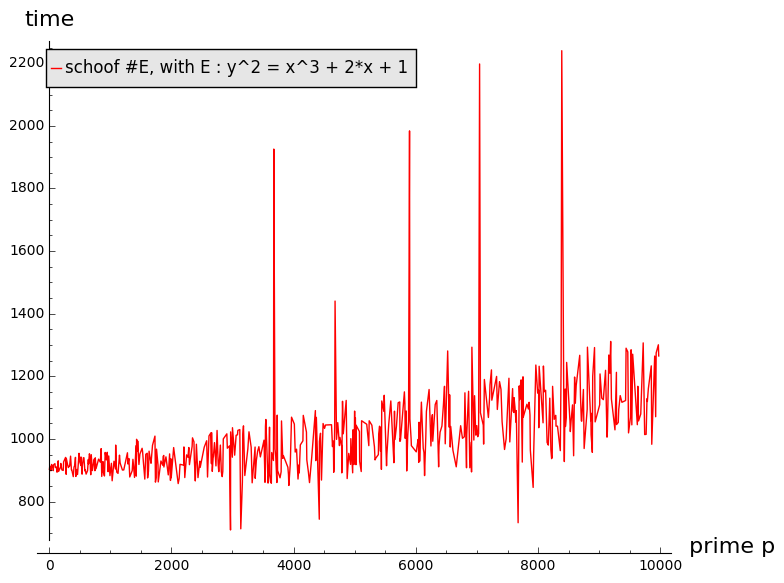
\includegraphics[scale=0.6]{pictures/schoof_cputime.png} 
\caption{Temps d'exécution de l'algorithme de Schoof}
\end{figure}

\begin{figure}[h!]
\caption{Comparaison temps exécution entre les algorithmes de Schoof et de brute force}
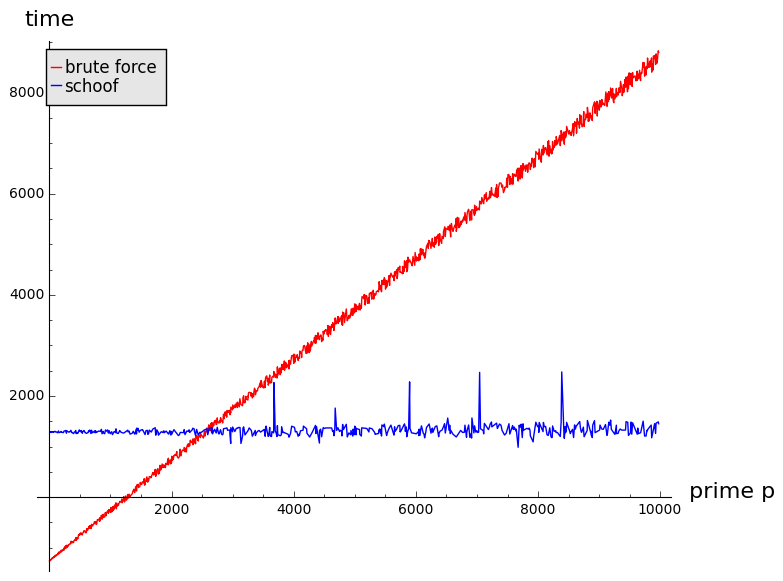
\includegraphics[scale=0.6]{pictures/schoof_vs_bruteforce.png} 
\end{figure}
On peut tirer deux informations intéressantes de ce graphique. D'une part on a confirmation que l'algorithme de Schoof est bien plus efficace que la méthode naïve dès que $p$ devient grand, mais on voit graphiquement que pour $p<2500$ il est plus efficace d'utiliser l'algorithme naïf.
\newline
Il est intéressant de se demander l'espace mémoire utilisé lors de l’exécution de l'algorithme de schoof, et vers quel quel $p$ premier on commence à atteindre des limites. Pour cela on va utiliser la plateforme Plafrim pour faire nos calcul....  (en attente des calculs). 
\newline
On a testé notre algorithme de Schoof sur une courbe du standard du NIST pour tester les limites de l'algorithme dans un cas réaliste. La courbe choisi est P-192 de paramètres :
\begin{align*}
p &= 6277101735386680763835789423207666416083908700390324961279\\
a &= -3 \\
b &= 1679885593
\end{align*}
On a du rajouter une option \path{sparsed=True} lors de la création de nos anneaux de polynômes pour permettre a SAGE de travailler avec des polynômes de très haut degré, il renvoyait une erreur overflow sinon. De plus le cas $l=2$ demande de calculer  $\gcd(x^p -x, x^3 - ax -b)$, ce qui sans algorithme efficace demande beaucoup trop de temps. Plutôt que d'essayer d’accélérer ce calcul le choix a été fait de simplement sauter le nombre premier $2$. De plus dans notre algorithme on test si le $l$-ième polynôme de division est irréductible ou non, s'il ne l'est pas on le remplace par l'un de ses facteurs. On utilise la fonction de SAGE \path{factor()} qui renvoie la factorisation de ce polynôme. Or si le degré devient important la factorisation notre polynôme va devenir plus longue que l’exécution complète de l'algorithme. On a uniquement besoin d'un seul facteur, pas de la décomposition entière, on pourrait donc optimiser cette étape.
......rajouter resultats des test ......
\subsubsection{Complexité}
La complexité de l'algorithme de Schoof est en $O(\log{q}^8)$ opérations élémentaires. La partie conteuse de l'algorithme réside dans les calculs dans l'anneau $R = \frac{\mathbb{F_p}[x,y]}{(f_l(x), y^2 -x^3 -ax -b)}$. Les éléments de R sont de degré $O(l^2)$ 
\newline
 L'algorithme est plus efficace qu'une version naïve quand la taille de $p$ augmente mais reste néanmoins limitée pour $p$ trop grand. En effet le degré des polynômes de division en $O(l^2)$ empêche une performance optimale pour des tailles de $p$ trop importante. Les polynômes de division deviennent rapidement très grands, ce qui pose un problème de mémoire. Une amélioration de cet algorithme a été proposée par Elkies-Atkin pour produire un algorithme plus performant, le SEA. 
 
\subsection{Algorithme SEA}
Il va être nécessaire d'introduire plus de théorie avant de s'attaquer à l'algorithme en lui même. L'idée finale est d'utiliser un polynôme de degré plus petit que les polynômes de division utilisés dans l'algorithme de Schoof, les polynômes modulaires. De plus pour comprendre certaines partie de l'algorithme SEA il va être nécessaire d'introduire un peu de théorie d'analyse complexe.


\subsubsection{Analyse complexe}
La théorie des courbes elliptiques est conséquente sur le corps des complexes mais nous allons uniquement donner des définitions et formules utiles, qu'on pourra retrouver ici \cite{complexbook} \cite{csi}, sans rentrer dans le détail de preuves et résultats non pertinents pour la compréhension de l'algorithme SEA. On peut légitimement se demander le rapport entre courbe elliptique et analyse complexe mais on va donc donner quelques définitions avant d'expliciter ce lien.

\begin{defi}
Une fonction holomorphe est une fonction à valeur complexe, définie et dérivable en tout point d'un sous ensemble ouvert du plan complexe $\mathbb{C}$. Une fonction est dite méromorphe si elle est holomorphe dans tout le plan complexe $\mathbb{C}$, sauf éventuellement sur un ensemble de points isolés dont chacun est un pôle pour la fonction.
\end{defi}

\begin{prop}
Soit $n \in \mathbb{N}$, $r \in \mathbb{R}$, $(w_i)_{1 \leq i \leq r}$ une partie libre du $\mathbb{R}$-espace vectoriel $\mathbb{R}^n$. Tout sous groupe discret non nul $\Gamma$ de $\mathbb{R}^n$ peut s'écrire sous la forme :
\begin{equation*}
\Gamma = \mathbb{Z} \omega_1 + \ldots + \mathbb{Z} \omega_r
\end{equation*}
Un tel groupe $\Gamma$ est un réseau de $\mathbb{R}^n$ de rang $r$.
\end{prop}
Dans le cas particulier de $\mathbb{C}$, ses sous-groupes discrets non nuls et non isomorphes à $\mathbb{Z}$ sont de la forme $\mathbb{Z}\omega_1 + \mathbb{Z}w_2$ avec $\omega_1, \omega_2 \in \mathbb{C}$ et $Im(\frac{w_2}{w_1}) \ne 0$. En pratique on va souvent considérer $\tau = \frac{\omega_2}{\omega_1}$ pour avoir $\Gamma = \mathbb{Z} + \tau \mathbb{Z}$.

\begin{defi}
On appelle tore le quotient $T = \mathbb{C}/ \Gamma$. C'est le quotient du groupe $(\mathbb{C}, +)$ par le réseau $\Gamma = \mathbb{Z}\omega_1 + \mathbb{Z}w_2$
\newline
Une fonction elliptique de période $\Gamma$ est une fonction méromorphe $f$ sur $\mathbb{C}$ telle que $f(z + \omega) = f(z) ,\ \forall \omega \in \Gamma$.
\end{defi}

\begin{defi}
Soit $\Gamma$ un réseau de $\mathbb{C}$, on introduit la $\wp$-fonction de Weierstrass par la série suivante :
\begin{equation*}
\wp(z) = \frac{1}{z^2} + \sum_{w \in \Gamma, \omega \ne 0} \frac{1}{(z-\omega)^2} - \frac{1}{\omega^2}
\end{equation*}
On a une convergence absolue donc uniforme sur tout compact disjoint de $\Gamma$ de cette série. De plus cette fonction est elliptique. On peut aussi définir sa dérivée ${\wp'}$ qui de même est elliptique :
\begin{equation*}
{\wp'} = -2 \sum_{\omega \in \Gamma} \frac{1}{(z-\omega)^3}
\end{equation*}
On peut montrer qu'avec $\Gamma = \omega_1 \mathbb{Z} + \omega_2 \mathbb{Z}$ cette fonction $\rho$ est doublement périodique de période $\omega_1, \omega_2$.
\end{defi}

Les théorèmes suivants permettent de faire le lien entre ces fonctions d'analyse complexe et les courbes elliptiques.

\begin{thm}
Soit $E$/$\mathbb{C}$ une courbe elliptique sous forme réduite sur le corps des complexes. Il existe alors un réseau $\Gamma$ tel que l'application suivante soit une bijection:
\newline
\medskip


$\begin{array}{cccc}
& \mathbb{C}\text{/ }\Gamma & \to & E \\
& z + \Gamma & \mapsto & \left\lbrace
\begin{array}{cc}
 (\wp(z), \frac{{\wp'}(z)}{2})  & z \notin \Gamma \\
 O & z \in \Gamma
\end{array}\right.\\
\end{array}$
\end{thm}

\begin{thm}
La fonction $\wp$ satisfait l'équation différentielle suivante : 
\begin{equation*}
{\wp'}(z)^2 = 4\wp^3(z) + A \wp + B
\end{equation*}
où les coefficients $A,B$ sont totalement déterminés en analysant les développements limités en $0$ de $\wp, {\wp'}$ et ${\wp'}^2$ et dépendent du réseau $\Gamma$.
\end{thm}

\subsubsection{Isogénie}
Soit $K$ un corps fini, on va noter dans la suite $E$/$K$ la courbe elliptique définie sur ce corps et on travaillera uniquement avec des courbes sous forme réduite.

\begin{defi}
Soit $E_1$/$K$ et $E_2$/$K$ deux courbes elliptiques. Si $E_1$ et $E_2$ ont le même $j$-invariant alors elles sont isomorphiques sur $\bar{K}$. 
\end{defi}
En d'autres termes, dire que deux courbes sont isomorphes signifie qu'il existe un changement de variable permettant de passer de l'une à l'autre. Avec un isomorphisme entre nos courbes, on peut s'intéresser à la structure des groupes des points rationnels de nos courbes, et à leurs relations.

\begin{prop}
Soit $E_1$/$K$ et $E_2$/$K$ deux courbes elliptiques isomorphes. On a alors un morphisme de groupe entre $E_1(K)$ et $E_2(K)$.
\end{prop}

\begin{defi}
Soit deux courbes elliptiques $E_1$ et $E_2$, $T_1=\mathbb{C}$/ $\Gamma_1$ et $T_2 = \mathbb{C}$/ $\Gamma_2$ les deux tores associés. Un morphisme de $E_1$ vers $E_2$ est une application holomorphe $\mu$ de $T_1$ vers $T_2$ qui soit un morphisme de groupe. Si ce morphisme est non constant alors on dit que c'est une isogénie.
\end{defi}

Deux courbes elliptiques $E_1$/$K$ et $E_2$/$K$ sont isogènes s'il existe une isogénie $\psi : E_1 \mapsto E_2$. Le degré de l’isogénie est le degré du noyau de $\psi$.


\subsubsection{Polynôme modulaire}
Ce sont les polynômes que l'on va utiliser dans l'algorithme SEA. Comme vu dans les parties précédentes on peut associer à chaque courbe elliptique $E$/$\mathbb{C}$ un invariant $\tau$ (on définissait un réseau $\Gamma = \mathbb{Z}+\tau \mathbb{Z}$), on a aussi $p=\e^{2\pi i \tau}$. De plus on peut exprimer le $j$-invariant de $E$ comme une série entière $j(p)$. Dans la suite on va noter $j(\tau) = j_E$.

La définition des polynômes modulaires est un peu plus compliquée qu'une simple formule, il nous faut définir, pour tout entier $n$, l'ensemble suivant : 
\begin{equation*}
S_n^* = \left\{ \begin{pmatrix}
a & b\\
0 & d
\end{pmatrix}
\, | \, a,b,d \in \mathbb{Z}, 0 \leq b \leq d, \gcd(a,b,d) = 1
 \right\} 
\end{equation*}
On peut définir la quantité suivante pour $\alpha \in S_n^* $:  $j \circ \alpha = j(\frac{a\tau +b}{d})$
On peut maintenant donner une définition des polynômes modulaires.

\begin{defi}
Soit $n$ un nombre premier, le $n$-ième polynôme modulaire est :
\begin{equation*}
\Phi_n(x,j) = \prod_{\alpha \in S_n^*} (x - j \circ \alpha)
\end{equation*}
\end{defi}
On peut noter que ce polynôme est à coefficients dans $\mathbb{Z}$, symétrique et de degré $n+1$ en chaque variable. De plus les coefficient de $x^{n+1}$ et $y^{n+1}$ sont $1$.
Ce qui nous permet de faire le lien entre isogénie et polynôme modulaire avec la définition suivante.
\begin{defi}
Soit $E_1$/$\mathbb{C}$ et $E_2$/$\mathbb{C}$ deux courbes elliptiques de $j$-invariant respectivement $j_{E_1}$ et $j_{E_2}$. Le $l$-ième polynôme modulaire vérifie $\Phi_l(j_{E_1},j_{E_2}) = 0$ si et seulement si il existe une isogénie entre $E_1$ et $E_2$ dont le noyau est cyclique de degré $l$.
\end{defi}

Ce théorème nous donne une méthode pour trouver toutes les isogénies à une courbe elliptique $E$/$\mathbb{F}_p$. Soit $l$ un nombre premier différent de $p$, on va chercher les racines de $\Phi_l(j_E, y) \in \mathbb{F}_p[y]$ dans $\mathbb{F}_p$. Quand on trouve une racine on trouve un j-invariant d'une courbe $E_2$ isogène avec $E$. 

On donne un exemple de polynôme modulaire, pour $ l =3$ on a :
\begin{align*}
\Phi_3(x,y) &= x^4 -x^3y^3 + y^4 \\
 +& 2232(x^3y^2 + x^2y^3) \\
 -& 1069956(x^3y^2 + x^2y^3 \\
 +& 36864000(x^3 + y^3) \\
 +& 2587918086x^2y^2 \\
 +& 8900222976000(x^2y + xy^2) \\
 +& 452984832000000(x^2 + y^2) \\
 -& 770845966336000000xy \\
 +& 1855000000000(x+y) 
\end{align*}
On peut noter que les coefficients augmentent très rapidement. Un algorithme efficace pour calculer ces polynômes dans le cas où $l$ est premier est le calcul via volcan d'isogénie \cite{volcan}

\subsubsection{Algorithme SEA}
Avec ce bagage théorique en plus on va pouvoir commencer à détailler l'algorithme SEA (schoof-Elkies-Atkins), on suppose dans la suite que $E$ est une courbe elliptique sous sa forme réduite $y^2 = x^3 + ax +b$ sur $\mathbb{F}_p$ avec $p$ premier . On rappelle que le polynôme caractéristique de l’endomorphisme de Frobenius $\phi$ sur $\mathbb{F}_l$ est $\chi_l(x) = x^2 - t_lx +p_l$ où $t_l$ est la trace du Frobenius modulo $l$, et $p_l$ la caractéristique du corps sur lequel on définit $E$ réduite modulo $l$. On va se demander si $\chi_l$ est irréductible sur $\mathbb{F}_l$. Or ce polynome a une racine dans $\mathbb{F}_l$ si et seulement si sont déterminant $\Delta_{\chi} = t_l^2 - 4p_l$ est un carré dans $\mathbb{F}_l$, ce qui nous amène à la classification suivante :

\begin{defi}
\label{Atkins's prime}
Si $\Delta_{\chi} = t_l^2 - 4p_l$ est un carré non nul dans $\mathbb{F}_l$ alors on dit que $l$ est un premier de Elkies, sinon c'est un premier de Atkins.
\end{defi}
\bigskip
On peut représenter graphiquement l'ensemble des points de $l$-torsions. On sait que l'on a $l^2$ points de $l$-torsion et que l'on peut décrire $E[l]$ par son $l$-ième polynôme de division $f_l$ de degré en $O(l^2)$.

\begin{tikzpicture}[>=latex]
\begin{axis}[
  axis x line=center,
  axis y line=center,
  title = {Représentation de $E[6]$},
  xtick={0,...,5},
  ytick={0,...,5},
  xticklabels={$0$,$P_1$, $2P_1$, $3p_1$, $4P_1$, $5P_1$},
  yticklabels={$0$,$P_2$, $2P_2$, $3p_2$, $4P_2$, $5P_2$},
  xmin=0,
  xmax=5.5,
  ymin=0,
  ymax=5.5]
\addplot[only marks] coordinates {
(0,0) (0,1) (0,2) (0,3) (0,4) (0,5) (1,0) (2,0) (3,0) (4,0) (5,0) (1,1) (2,2) (3,3) (4,4) (5,5) (1,2) (1,3) (1,4) (1,5) (2,1) (2,3) (2,4) (2,5) (3,1) (3,2) (3,4) (3,5) (4,1) (4,2)
(4,3) (4,5) (5,1) (5,2) (5,3) (5,4) 
};
\end{axis}
\end{tikzpicture}

L'idée de l'algorithme SEA est de ne plus travailler sur cet ensemble $E[l]$ mais sur l'un de ses sous groupe contenant $l$ points et décrit par un polynôme $g_l$ divisant $f_l$ mais cet fois de degré en $O(l)$.
\newline
\bigskip
\begin{tikzpicture}[>=latex]
\begin{axis}[
  axis x line=center,
  axis y line=center,
  title = {Représentation d'un sous groupe de $E[6]$},
  xtick={0,...,5},
  ytick={0,...,5},
  xticklabels={$0$,$P_1$, $2P_1$, $3p_1$, $4P_1$, $5P_1$},
  yticklabels={$0$,$P_2$, $2P_2$, $3p_2$, $4P_2$, $5P_2$},
  xmin=0,
  xmax=5.5,
  ymin=0,
  ymax=5.5]
\addplot[only marks] coordinates {
(0,0) (1,1) (2,2) (3,3) (4,4) (5,5) 
};
\end{axis}
\end{tikzpicture}

On peut noter que $E[l]$ contient $l+1$ sous groupe cyclique d'ordre $l$.
La question est donc quel sous groupe prendre ? On va s’intéresser à un sous espace propre de la restriction de $\phi$ à $E[l]$ de dimension $1$ (comme visible sur le graphique précédent on prend une droite) qu'on note $C_{\lambda}$. La valeur propre associée à ce sous espace propre est bien sur $\lambda$ tel que $\phi(P) = \lambda P$ pour $P \in C_{\lambda}$. On décrit $C_{\lambda}$ par $g_l$.
\newline
On peut décrire $\phi_{|E[l]}$ par une matrice $2\times2$, la question de trouver des sous espace propre est liée a la question de diagonalisation de cette matrice.

Atkins a montré qu'a partir des polynômes modulaire on peut déterminer si $\Delta_{\chi}$ est un carré. Il en résulte le théorème suivant:

\begin{thm}
\label{thm calcul r}
Soit $E$ une courbe elliptique définie sur $\mathbb{F}_p$ de $j$-invariant non nul. On note $\Phi_l(j,y) = h_1(y) \ldots h_s(y)$ la factorisation du $l$-ième polynôme modulaire sur $\mathbb{F}_p[y]$ en produit de polynôme irréductible. On a alors les possibilités suivantes pour les degrés de $h_1, \ldots, h_s$:
\begin{itemize}
\item[(1)] $(1,l)$ ou $(1,\ldots,1)$, dans les deux cas $\Delta_{\chi} \equiv 0 \pmod l$, et on pose respectivement $r=l $ et $r=1$.
\item[(2)] $(1,1,r,\ldots,r)$, dans ce cas $\Delta_{\chi}$ est un carré dans $\mathbb{F}_l$, $r$ divise $l-1$ et $\phi_l$ agit sur $E[l]$ comme la matrice diagonale $\begin{pmatrix}
\lambda & 0 \\
0 & \mu
\end{pmatrix}$ avec $\lambda,\mu \in \mathbb{F}_l^*$.
\item[(3)] $(r, \ldots, r)$ pour $r>1$, dans ce cas $\Delta_{\chi}$ n'est pas un carré dans $\mathbb{F}_l$, $r$ divise $l+1$ et $\chi_l$ est irréductible sur $\mathbb{F}_l$.
\end{itemize}

Dans tous les cas $r$ est l'ordre de $\phi_p$ dans le groupe projectif linéaire $PGL(\mathbb{F}_l)$ et la trace du Frobenius satisfait : 
\begin{equation}
\label{trace with root of unity}
t^2 \equiv p(\xi+\xi^{-1})^2 \pmod l
\end{equation}
Où $\xi$ est une $r$-ième racine primitive de l'unité dans $\bar{\mathbb{F}_l}$.
\end{thm}
 On rappelle que le $PGL(E)$ d'un espace vectoriel $E$ sur un corps $K$ est le groupe quotient $GL(E)$/$Z(E)$. Où $GL(E)$ est le groupe général linéaire de $E$, le groupe des automorphismes de $E$ muni de la composition des applications. Et $Z(E)$ le centre de $GL(E)$, c'est a dire l'ensemble des éléments de $E$ qui commutent avec tous les autres.
\newline
On peut reformuler la classification énoncée dans la définition \ref{Atkins's prime}. Un nombre premier $l$ tel que $\phi_{|E[l]}$ est diagonalisable est un premier de Elkies, et un premier de Atkins sinon. Pour déterminer dans quel cas on se trouve on va étudier la factorisation de $\Phi_l(x,j)$ ($j$ est le $j$-invariant de notre courbe elliptique $E$). Pour se faire on va calculer le degré de $\gcd(\Phi_l(x,j),x^p-x)$, d'après le théorème précédent si ce $\gcd$ est constant alors $l$ est un premier d'Atkins, sinon c'est un premier d'Elkies.


\paragraph*{Premier d'Elkies}
On se place dans le cas ou $l$ est un premier d'Elkies. Le Frobenius est diagonalisable, de valeurs propres $\lambda, \mu$, car $\Delta_{\chi_l} =t_l^2 -4p$ est un carré modulo $l$ (on rappelle que $\chi_{l}(x) = x^2 - t_lx +p_l$). Ainsi on a :
\begin{equation*}
\chi_l(x) = (x - \lambda)(x- \mu)
\end{equation*}
Donc $t_l \equiv \lambda +\mu \equiv \lambda + \frac{p_l}{\lambda} \pmod l$ (car $p_l = \lambda\mu$). On peut la trace modulo $l$ en trouvant une valeur propre du Frobenius. La première question est de se demander si $\lambda \ne \mu$, si on est dans ce cas alors $t_l = 2 \lambda = 2 \sqrt{p_l}$ et on se ramène à un cas expliqué dans la partie sur l'algorithme de Schoof. Le cas le plus intéressant est donc quand $\lambda \ne \mu$. Par définition d'une valeur propre on sait qu'il existe deux points $P_1,P_2 \in E[l]$ non triviaux tel que $\phi_p(P_1) = [\lambda]P_1$ et $\phi_p(P_2) = [\lambda]P_2$. Soit $C_1$ et $C_2$ les deux sous groupes cyclique d'ordre $l$ générés par $P_1$ et $P_2$, ils sont stables par l'action du Frobenius, c'est à dire $\phi_p(C_1) = C_1$. On peut alors construire le polynôme $g_l$ de degré $\frac{(l-1)}{2}$ et divisant le $l$-ième polynôme de division : 
\begin{equation}
\label{poly g_l}
g_l(x) = \prod_{\pm P \in C_1^*} (x - x_p), \quad \text{où } P = (x_p, y_p)
\end{equation}
On peut à partir de ce polynôme utiliser l'algorithme de Schoof pour trouver la trace du Frobenius modulo $l$. On commence par noter que vu que $\lambda$ est valeur propre, pour tout point de $C_1$  on a l'équation $\phi(P) = [\lambda]P$. On peut appliquer nos formules de multipication scalaire énoncé dans notre partie sur les polynomes de division. L'abscisse du point [$\lambda$]$P$ est : 
\begin{equation*}
x - \frac{\psi_{\lambda-1}\psi_{\lambda+1}}{\psi_{\lambda}^2}
\end{equation*}
Avec $\phi(P)=(x^p,y^p)$ on trouve :
\begin{equation*}
x^p = x - \frac{\psi_{\lambda-1}\psi_{\lambda+1}}{\psi_{\lambda}^2}
\end{equation*}
On pose $h(x) = \psi_{\lambda}^2(x^p-x) + \psi_{\lambda-1}\psi_{\lambda+1}$, qu'on réduit modulo $g_l$. Il faut trouver une valeur propre $\lambda$ tel que $\gcd(h,g_l) \ne 1$. Une fois que l'on a trouvé une valeur qui correspond on peut calculer $t_l = \lambda + \frac{p_l}{\lambda} \pmod l$

Il faut maintenant montrer comment construire ce polynôme $g_l$. L'idée va être de trouver dans un premier temps le premier coefficient de $g_l$ (qui est moins la somme des racines de $g_l$). On sait que le degré du polynôme $\gcd(\Phi(x,j),x^p-x)$ est plus grand que $0$ comme $l$ est un premier de Elkies et que ses racines sont dans $\mathbb{F}_p$. Notons par exemple $\tilde{j}$ l'une de ses racines. On sait donc qu'il existe une isogénie entre $E$ et la courbe elliptique de $j$-invariant $\tilde{j}$ qu'on note $\tilde{E}:y^2=x^3+\tilde{a_4}x+\tilde{a_6}$. Le noyau de cette isogénie est l'un des $l+1$ sous groupe cyclique de $E[l]$. On va utiliser cette isogénie pour retrouver le premier coefficient de $g_l$. On ne détaillera pas les calculs permettant d'arriver a ce résultat, ils s'appuient fortement sur l'analyse complexe évoqué plus haut. Plus d'informations peuvent être trouver ici \cite{sea}.


\paragraph*{Premier d'Atkin}
On va étudier le degré $r$ de $\phi_p$ dans $PGL_2(\mathbb{F}_l)$. Il faut dans un premier temps déterminer le plus petit $i>1$ tel que : 
\begin{equation}
\gcd(\Phi_l(x,j), x^{p^i} - x) = \Phi_l(x,j)
\end{equation}
On recherche donc la plus petite extension $\mathbb{F}^{p^i}$ de $\mathbb{F}_p$ contenant toutes les racines de $\Phi_l(x,j)$. Ce $i$ est alors le degré de $\phi_p$, et on peut montrer qu'il suffit de tester les $i$ divisant $l+1$ et qui satisfont $(-1)^{\frac{l+1}{i}}= (\frac{p}{l})$. On rappelle qu'on a une relation entre les racines primitives de l'unité et la trace d’après l'équation \ref{trace with root of unity}. On va construire un ensemble de valeurs possibles pour la trace modulo $l$. Soit $\lambda$ et $\mu$ deux valeurs propre de $\phi_p$, alors $\gamma = \frac{\lambda}{\mu}$ est une $r$-ième racine primitive de l'unité et $\gamma \in \mathbb{F}_{l^2}$. On peut aussi écrire, pour $d$ qui n'est pas un carré de $\mathbb{F}_l$, $\mathbb{F}_{l^2} \cong \mathbb{F}_l[\sqrt{d}]$. On peut alors énumérer toute les valeurs de $\gamma$. Soit $g$ un générateur de $\mathbb{F}_{l^2}$ alors $\gamma = g^{\frac{l^2-1}{r}}$ est une $r$-ième racine de l'unité, pour trouver les autres on calcule $\gamma_i = \gamma^i$. Montrons maintenant comment utiliser ces $\gamma_i$ pour calculer notre ensemble de trace. Sans détailler, l'idée est d'écrire $\gamma_i$ sous la forme $\gamma_i = g_{i_1} + g_{i_2}\sqrt{d}$ avec $g_{i_1}, g_{i_2}$ dans $\mathbb{F}_l$, mais on peut aussi montrer que pour $x_1, x_2 \in \mathbb{F}_l$ on a $\lambda = x_1 + x_2\sqrt{d}$ et $\mu = x_1-x_2\sqrt{d}$. En utilisant la relation $\gamma_i = \frac{\lambda}{\mu}$. Les $x_i$ sont inconnu mais pas les $g_{i}$, au final on a la relation $x_1^2 = \frac{p(g_{i_1}+1)}{2}$. Si $x_i^2$ n'est pas un carré dans $\mathbb{F}_l$ on passe au $\gamma_i$ suivant, sinon sachant que $t \equiv \lambda + \mu = 2x_1$ on ajoute à notre ensemble de trace $2x_1$ et $-2x_1$.


\paragraph*{Retrouver $t$}
On ne peut pas simplement utiliser les restes chinois comme pour l'algorithme de Schoof. En effet la trace que l'on trouve en utilisant les premiers d'Atkins est un ensemble de traces possibles, on n'a pas unicité. Plusieurs possibilités sont possible, la plus simple mais peut etre moins efficace est de considérer plus d'entier $l$ pour calculer notre trace modulo $l$. L'autre idée est d'utiliser un algorithme baby-step/giant-step qui sera plus efficace.

\newpage
\subsubsection{Algorithme pseudo-code}
On donne une description en pseudo-code de l'algorithme SEA.
\begin{algorithm}
\caption{Schoof-Elkies-Atkins}
\begin{algorithmic}
\REQUIRE $E$ une courbe elliptique de la forme $y^2 = x^3 + ax = b$ sur $\mathbb{F}_p$
\ENSURE Le nombre de points de $E$
\STATE Calculer le $j$-invariant de $E$
\STATE Choisir un ensemble de premier S tel que $\prod_{l \in S}l \leq 4\sqrt{p}$
\FORALL{$l \in S$}
\IF{$deg(\gcd(\Phi_l(x,j),x^p-x)=0$)}
\STATE Calculer $r$ avec le théorème \ref{thm calcul r}
\STATE Calculer $d$ tel que $(\frac{d}{l}) = -1$, et $0<d<l$
\STATE Calculer $g$ tel que $g$ soit un générateur de $\mathbb{F}_l[\sqrt{d}]^*$
\STATE Calculer $S_2 = \left\{g^{\frac{i(l^2-1)}{r}} \, | \, \gcd(i,r) = 1 \right\}$
\FORALL{$\gamma \in S_2$}
\STATE écrit $\gamma_i = g_{i_1} + \sqrt{d}g_{i_2}$
\STATE Calculer $z= \frac{p(g_{i_1} +1)}{2} \pmod l$
\IF{$(\frac{z}{l})=1$}
\STATE Calculer $x = \sqrt{z} \pmod l$
\STATE $t_l = (2x,-2x)$
\ENDIF
\ENDFOR
\ELSE
\STATE Calculer $g_l$ un diviseur de $f_l$
\STATE Trouver $\lambda$ valeur propre du Frobenius tel que $\gcd(\psi_{\lambda}^2(x^p-x) + \psi_{\lambda-1}\psi_{\lambda+1}, g_l(x)) \ne 1$
\STATE Calculer $t = \lambda + \frac{\lambda}{p} \pmod l$
\ENDIF
\ENDFOR
\STATE retrouver $t$ en utlisiant les $t_l$ 
\STATE retourner $p+1-t$
\end{algorithmic}
\end{algorithm}

\paragraph*{Complexité}
L'algorithme SEA a une complexité heuristique de $O(\log^4 p)$ en temps, et $O(\log^2 p)$ en espace.

\newpage
\bibliographystyle{plain}
\bibliography{biblio}

\end{document}